\section{Drift Chamber Tracking System Performance}

In this section, we describe the tracking system performance: the ability to operate at high luminosity,
the efficiency at reconstructing charge particle tracks, and the spatial resolution of such tracks.

\subsection{Operation at High Luminosity}

In order to satisfy the statistical requirements of the experimental program, an important design
goal for CLAS12 is the ability to make routine measurements with electron beam luminosities up to
10$^{35}$~cm$^{-2}$s$^{-1}$.  The luminosity limit in CLAS12 is 
set by the large flux of M{\o}ller electrons and low-energy photons 
produced from the targets by the multi-GeV incident electron beam.  This 
constraint is severe for the drift chambers since they are close to the 
target. 

Particularly for the R1 chambers, the large flux of particles limits the luminosity in several ways.
First, the chambers must be able to operate with an acceptably low trip rate.
Second, the accidental occupancy in the chambers should be on the order
of 5\% or less in order to keep the track-finding inefficiencies at a moderate 
level.  See the accompanying article on track reconstruction (\cite{recon-nim})
for a quantitative discussion of this effect.  Third, the effects of sustained high 
luminosities can be unfavorable for long chamber lifetimes.  Aging correlates 
directly with the currents generated in the chambers.
However, our choice of an argon-CO$_2$ gas mixture and strict control of
materials in contact with the gas should provide a long chamber lifetime.
For the previous CLAS chambers, we used the same gas mixture and ran at a
similar gain and similar currents, and the chambers lasted more than 10 years 
with no indication of aging.  We expect the present
chambers to perform well for at least 10 years.

\subsection{Tracking Inefficiency: Intrinsic, Malfunction-Related, and Background-Related}

The probability of reconstructing a track due to a charged particle within our fiducial volume
is referred to as the ``tracking efficiency''. The tracking inefficiency has three root causes:

\begin{enumerate}
\item {\bf intrinsic layer inefficiency}: the failure to record
a hit for a track crossing a layer, when all wires and electronics
are operating properly;
\item {\bf malfunction-related inefficiency}: loss of hits and sometimes
whole track segments because of equipment malfunctions;
\item {\bf background-related inefficiency}: out-of-time background
can interfere with the segment-finding algorithms when a background-related
track segment lies ``on top'' of a real, in-time, segment.
\end{enumerate}

\subsubsection{Simulation of Inefficiencies}

In our generation and reconstruction of simulated events, we estimate the size of
the three types of inefficiency in the following manner:

\begin{enumerate}
\item {\bf simulation of intrinsic layer inefficiency}: this is a random process
and, as such, it is handled at event generation time by our Monte Carlo simulation
program GEMC~\cite{sim-nim}.  For each superlayer (1-6), we have defined a DOCA-dependent
layer inefficiency function, as determined from the data.  At hit-generation
time in GEMC a random number (between 0 and 1) is generated, and if it is
smaller than the layer inefficiency function, the hit is not digitized.
\item {\bf simulation of malfunction-related inefficiency}: the GEMC Monte
Carlo hits are generated as if there are no malfunctions of the wires.
During the Monte Carlo reconstruction, however, a status table for each
hit wire is queried and if the wire is in the ``bad status'' list, that
hit is not used in the tracking.  The malfunction-related inefficiency  is small.  
At the time of publication, roughly $0.5\%$ of our wires are not operating properly.  
\item {\bf simulation of background-related inefficiency}: rather than try
to simulate out-of-time background due to all physics processes, we merge
``random-trigger'' events with events from low-luminosity runs and compare the
efficiency of these merged events with that from un-merged low-luminosity events.
This ratio is considered to be a measure of the background-related inefficiency.
\end{enumerate}

We will not further discuss the {\bf malfunction-related inefficiency} or
the {\bf background-related inefficiency} further in this article.  See
our companion article on track reconstruction for more details~\cite{recon-nim}.

Here we present our results on measuring the {\bf intrinsic layer inefficiency}.

\subsubsection{Intrinsic Layer Inefficiency}

The layer efficiency is the probability that a
good hit is recorded in a wire layer through which the track has passed, based on 
the evidence from all other layers in the superlayer.  This is called the 
``excluded-layer method''.  The layer efficiency is a measure of the intrinsic drift 
cell efficiency for the particular choice of gas mixture, high-voltage set point, and 
discriminator level.  

The single layer inefficiency is not uniform across the drift cell.  It is slightly higher near the sense 
wire and substantially higher near the outer edge of the cell.  A track passing close to a sense wire 
leaves many ions in the cell, but the
ion arrival times are stretched out from near-zero to the maximum drift time $Tmax$.  The result is that
the preamplifier's output signal has a low voltage amplitude but persists for a long time.  So, even though
the collected charge is large the voltage put out by our transimpedance preamplifiers may not be large
enough to exceed the voltage discriminator threshold of the DCRB. For the case of tracks near the outer
edge of the cell (so-called `corner-clippers') they leave a very small number of ions in the cell and
thus have a small signal.

Fig.~\ref{dc-inefficiency-vs-doca} shows that the largest contribution to the drift cell
inefficiency is from tracks far from the wire.  These tracks may leave very few ions,
so -called 'corner clippers'.  Even tracks that are far from the wire but leave a substantial
number of ions can give rise to inefficiencies due to a large spread in ion arrival time.  
These tracks produce signals 
that have low pulse height and long duration, and thus may escape detection.
We fit this observed DOCA-dependent inefficiency to a functional form that is
used in our GEMC Monte Carlo hit digitization routine to randomly throw out
this percentage of hits.

%%%%%%%%%%%%%%%%%%%%%%%%%%%%%%%%%%%%%%%%%%%%%%%%%%%%%%%%%%%%%%%%%
\begin{figure}[htbp]
\vspace{7cm}
\begin{picture}(50,50)
\put(0,0)
{\hbox{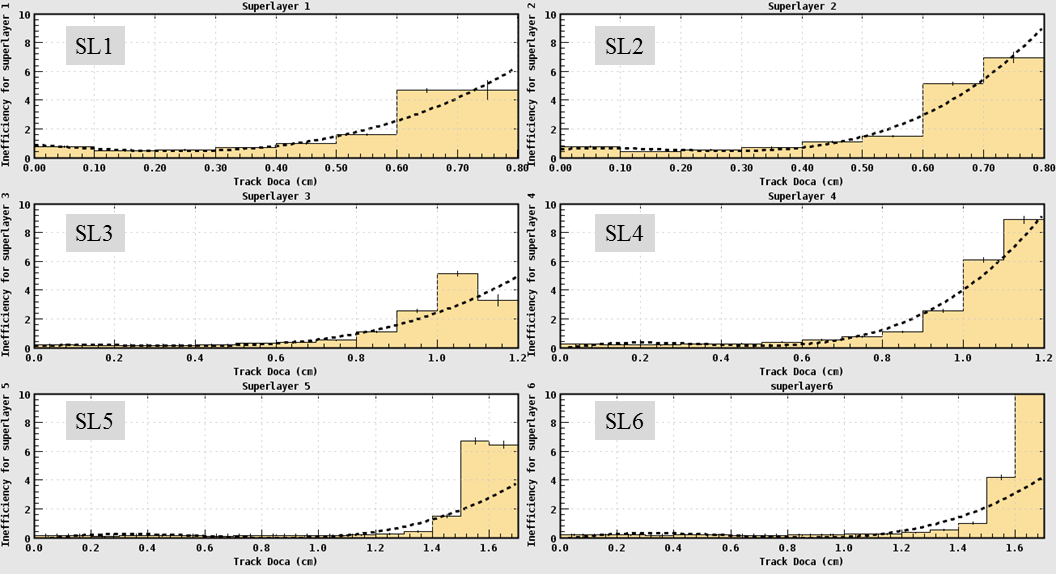
\includegraphics[width=0.8\textwidth,natwidth=610,natheight=642]{img/dc-inefficiency-vs-doca.png}}}
\end{picture}
\caption{\small{The observed ``layer efficiency'' as a function of DOCA.  Hits from tracks
that pass close to or far from the sense wire have the hits spread out in time, and the resulting
voltage pulse from the preamplifiers may fail to cross the discriminator threshold, resulting
in a ``lost hit''.}}
\label{dc-inefficiency-vs-doca}
\end{figure}
%%%%%%%%%%%%%%%%%%%%%%%%%%%%%%%%%%%%%%%%%%%%%%%%%%%%%%%%%%%%%%%%%%%

\subsection{Drift Chamber Spatial Resolution}

The single-wire resolution is the RMS spread of the difference 
between the fitted TRKDOCA of the track and the value of DOCA as calculated from the 
time of the hit.  The variance of this residual distribution 
is the quadratic sum of the single-wire resolution and the track position uncertainty.  
This variance over-estimates the single-wire resolution.
Since there are six layers per superlayer,
this amounts to a $10 - 15\%$ over-estimate.

Fig.~\ref{resolution-vs-doca} shows the width of the track-hit residual distribution plotted versus
TRKDOCA for each of the different chamber regions.  The single-wire resolution worsens near the 
wire and also at the outer edge of the cell.  This arises due to finite cluster sizes 
due to the Poisson distribution of ion-pair production along the path of the primary ion 
near the sense wire along with time walk effects and the divergent nature of the electric
field lines near the field wire.  

%%%%%%%%%%%%%%%%%%%%%%%%%%%%%%%%%%%%%%%%%%%%%%%%%%%%%%%%%%%%%%%%%
\begin{figure}[hbtp]
\vspace{7.3cm}
\begin{picture}(50,50)
\put(50,-10)
{\hbox{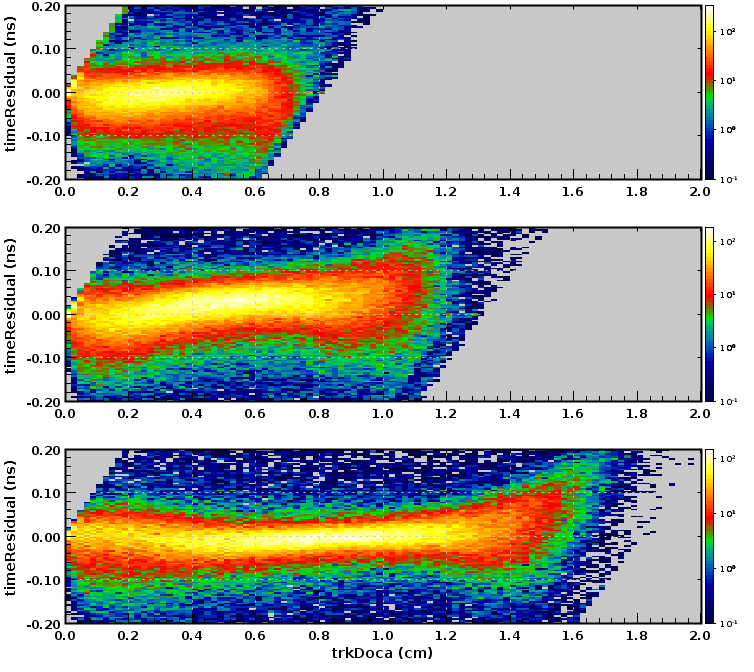
\includegraphics[width=0.85\textwidth,natwidth=610,natheight=642]{img/resolution-vs-doca.png}}}
\end{picture}
\caption{\small{The hit resolution plotted versus TRKDOCA for R1, R2, and R3 (top, middle, bottom),
    respectively.}}
\label{resolution-vs-doca}
\end{figure}
%%%%%%%%%%%%%%%%%%%%%%%%%%%%%%%%%%%%%%%%%%%%%%%%%%%%%%%%%%%%%%%%%%%

A more quantitative look at the resolution is given in Fig.~\ref{gaussian-fit-to-resids}.
This is a plot of the residual distributions from each of the six superlayers in Sector 1; 
all sectors have similar results.
Because the resolution is narrow in the middle of the cell and widens considerably
for small and large values of DOCA (see Fig.~\ref{resolution-vs-doca}), we fit the
residual distribution to a double-Gaussian form. 
The average single-wire resolution in the middle 
portion of the cell is about 325, 395 or 310~$\mu$m for R1, R2 and R3, respectively,
with a whole cell resolution (RMS) of about 430, 540 or 515~$\mu$m for R1, R2 and R3, respectively.

%%%%%%%%%%%%%%%%%%%%%%%%%%%%%%%%%%%%%%%%%%%%%%%%%%%%%%%%%%%%%%%%%
\begin{figure}[htbp]
\vspace{7cm}
\begin{picture}(50,50)
\put(0,-5)
{\hbox{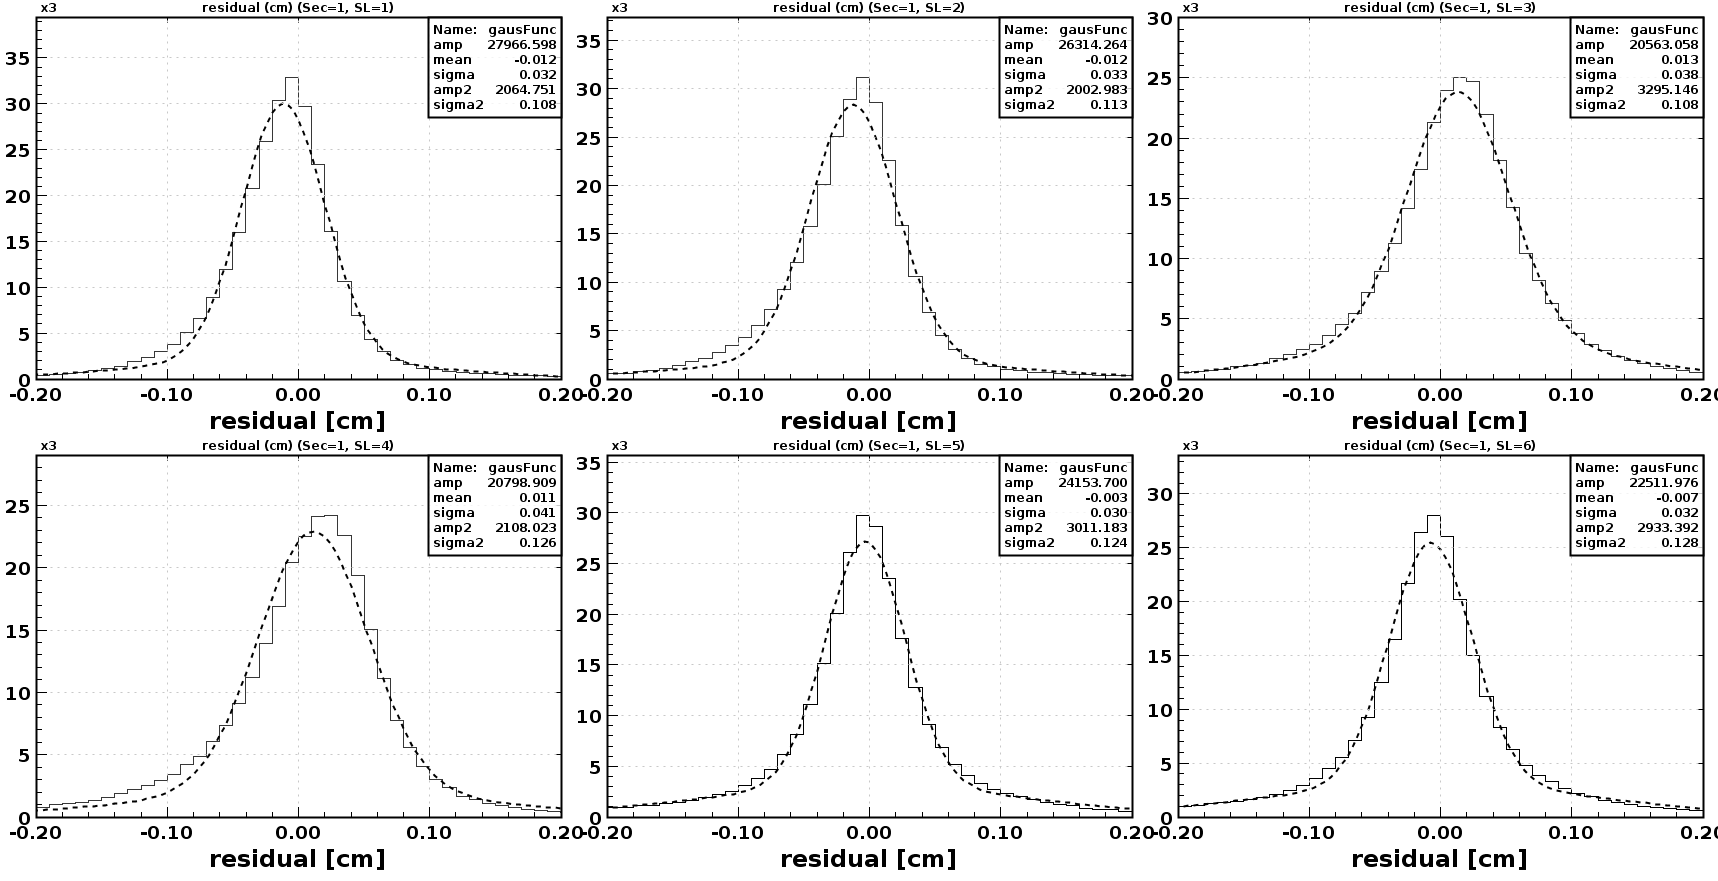
\includegraphics[width=.5\textwidth,natwidth=610,natheight=642]{img/gaussian-fit-to-resids.png}}}
\end{picture}
\caption{\small{A plot of the residual distributions for all 6 superlayers in Sector 1.  Overplotted
is a double-Gaussian fit to the distribution.}}
\label{gaussian-fit-to-resids}
\end{figure}
%%%%%%%%%%%%%%%%%%%%%%%%%%%%%%%%%%%%%%%%%%%%%%%%%%%%%%%%%%%%%%%%%%%

\subsection{Summary of Design, Construction and Operation}

The toroidal geometry of the CLAS spectrometer necessitated a particle-tracking 
system of unconventional design.  Design challenges and solutions include the following:

\noindent
- The necessity to conceal inactive areas of the drift chambers within the
shadow regions of the torus cryostat resulted in very thin endplates and low-profile
wire connection schemes and on-board preamplifiers.

\noindent
- The toroidal shape of the magnet and the desire to have measurements before, within, 
and after the high-field region, resulted in the design of a ``rod and ball'' mounting scheme
that minimizes dead areas and facilitates maintenance.

\noindent
- The fabrication of chambers that support large static wire tensions, but have thin 
endplates necessitated three endplate designs: aluminum stiffened with steel bars (R1),
Stesalit (an epoxy-G10 composite) stiffened with steel bars (R2), and thin stainless-steel 
plates filled with foam and reinforced
with carbon-fiber posts on the entrance side and a carbon-foam-carbon composite plate on the exit side (R3). 

\noindent
-The need for precise tracking in a system with non-saturated drift velocity 
(necessitated by the requirements of large drift distances, non-flammable gas mixtures, 
and low-gain operation) resulted in a semi-automated calibration and monitoring software 
package.

\vskip 10pt
\subsection{Conclusions}
The CLAS12 drift chamber system has been in routine operation since spring, 2017. 
The system has reached its design goals of high-luminosity operations
(1$\times$10$^{35}$~cm$^{-2}$s$^{-1}$) in a high-flux electromagnetic reaction
environment, with very good track reconstruction efficiency over a large range of angles and 
magnetic fields; see the article on track reconstruction~\cite{recon-nim}.  
The percentage of malfunctioning wires, due to high voltage problems, signal
connector issues, etc., is presently ~0.5\%.
The single-wire efficiency is greater than $98\%$ and the
single-wire resolution is about 400~$\mu$m averaged over all drift distances and
all 18 chambers, with each chamber showing a characteristic 250~$\mu$m resolution 
in the cell center.

\vskip 10 pt

{\large{\bf Acknowledgments}}

\vskip 10pt

The authors wish to thank the crews of wire stringers and technicians who 
participated during the chamber construction at the Idaho State University,
Old Dominion University, and Jefferson Laboratory, as well as the support of 
the technicians involved with installation of the detectors into CLAS12.  The
authors also thank Dr. Simon Taylor for his careful reading of the draft.  This
work was supported in part by DOE contract DE-AC05-84ER40150, DOE grants 
DE-FG02-87ER40315, DE-FG05-94ER40859, DE-FG02-96ER40960, DE-FG02-96ER40980, 
and NSF grant NSF-PHY-9412479.




